% PROTOKOLL Action Item
\documentclass[
   draft=false
  ,paper=a4
  ,twoside=false
  ,fontsize=11pt
  ,headsepline
  ,DIV11
  ,parskip=full+
]{scrartcl} % copied from Thesis Template from HAW

\usepackage[ngerman,english]{babel}
\usepackage[T1]{fontenc}
\usepackage[utf8]{inputenc}

\usepackage[
    left  =4em
   ,right =4em
   ,top   =5em
   ,bottom=5em
]{geometry}

\usepackage{longtable}
\usepackage[german,refpage]{nomencl}

\usepackage{float}
\usepackage{enumitem}
\usepackage{hyperref} % for a better experience

\hypersetup{
   colorlinks=true % if false - links get colored frames
  ,linkcolor=black % color of tex intern links
  ,urlcolor=blue   % color of url links
}

\usepackage{graphicx}
\usepackage{amsmath}

\usepackage{array}   % for \newcolumntype macro
\newcolumntype{L}{>{$}l<{$}} % math-mode version of "l" column type
\newcolumntype{R}{>{$}r<{$}} % math-mode version of "r" column type
\newcolumntype{C}{>{$}c<{$}} % math-mode version of "c" column type

\usepackage{listings}
\lstset{language=C} 
\usepackage{caption}
\usepackage{colortbl}
\definecolor{tabgrey}{rgb}{0.85,0.85,0.85}
%using minted because of the hashtag in bash

\sloppy
\clubpenalty=10000
\widowpenalty=10000
\displaywidowpenalty=10000

\begin{document}

\selectlanguage{ngerman}
% ----------------------------------------------------------------------------
% ---------------------------------------------------------- HIER WAS MACHEN -
% -------------------------------- Metadaten wie namen und Gruppentreffen etc-
\def\titel{AD Praktikum: Aufgabe 09, Graph and Dykstra}


\def\teilnehmer{ 
	& Sönke Peters & \\
    & Karl-Fabian Witte   & \\
}
% -------------------------------------------------- HIER AUFHÖREN ----------




% ------------------------------------------ einige strukturell Definitionen
\newlength{\txtw} %definiere neue länge
\setlength{\txtw}{\textwidth} %setze neue länge auf textbreite
\addtolength{\txtw}{-10\tabcolsep} %subtrahiere -8\cdot textbreite von asdf

\def\me{\myName \newline \footnotesize{\url{\myEmail} } }

% ------------------------------------------------------------------ Inhalt	
\section*{\titel}
\begin{tabular}{l p{0.4\txtw} p{0.4\txtw} }
	\teilnehmer
	& & \\
	& \today & \\
\end{tabular}


\centering
\textbf{Abstract} \\
Die Datenstruktur eines gewichteter Graphen wird auf Adjazenzmatrix und -liste implementiert und der Algorithmus von Dykstra wird auf diesen mit 
einer Komplexitätsuntersuchung ausgewertet. 
\normalsize \flushleft
\section{Aufgabenstellung}
Es sollen zwei Implementationen von dem abstrakten Datentyp Graph 
realisiert werden. Die Komplexität des Dykstras Algorithmus 
ist auf beiden Graphenimplementationen zu messen. Die für den 
Algorithmus wichtigen zusatzinformationen sind nicht im Graphen
selbst gespeichert. 
Zudem sollen zufallsgeneriertere Graphen erstellt werden, welche 
für die Messung der Komplexität verwedet werden.

\subsection{Grapheninterface und Implementationsarten}
\begin{figure}[htp]
  	\centering
    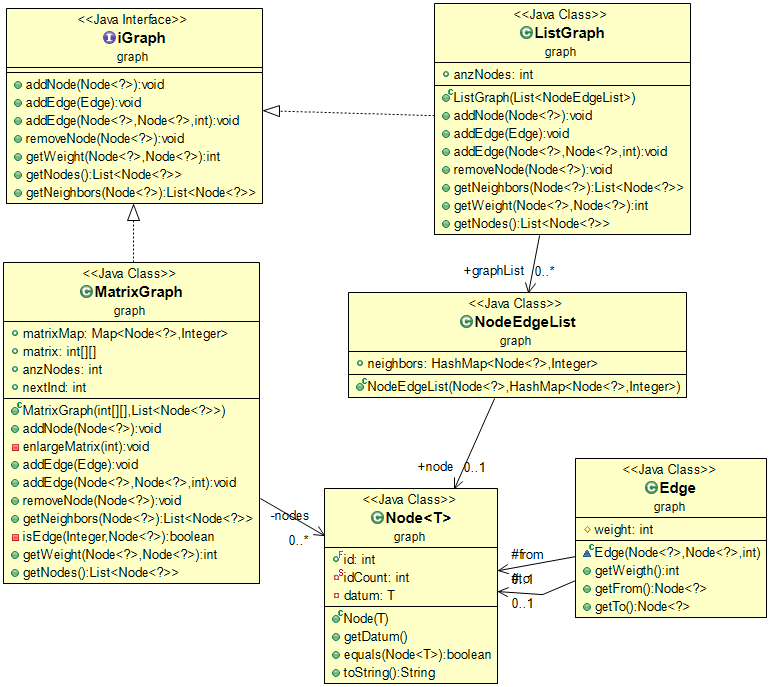
\includegraphics[width=\textwidth]{./IMG/graph.png}
    \caption[shortone]{UML Diagramm, der Implementation der Graphendarstellungen}
    \label{fig:plot}
\end{figure}

\subsubsection{Adjazenzmatrix}

Eine Adjazenzmatrix eines Graphen ist eine Matrix, die speichert, welche Knoten des Graphen durch eine Kante verbunden sind. Sie besitzt für jeden Knoten eine Zeile und eine Spalte, woraus sich für n Knoten eine n$\times$n-Matrix ergibt. Ein Eintrag in der i-ten Zeile und j-ten Spalte gibt hierbei an, ob eine Kante von dem i-ten zu dem j-ten Knoten führt. Steht an dieser Stelle eine -1, ist keine Kante vorhanden. Steht an dieser Stelle eine 0, ist keine Kante vorhanden, da der Knoten sonst eine Kante auf sich selbst führen würde, was wir ausschließen. Ist der Wert größer als 0 so gibt er die Kosten für diesen Weg an.

\subsubsection{Adjazenzliste}
Eine Adjazenzliste eines Graphen ist eine Liste, die speichert, welche Knoten des Graphen durch eine Kante verbunden sind.
Jeder Knoten hat seine eigene Liste, die seine Nachbarn beinhaltet.
In unserem Fall speichert die Liste außerdem noch die Kosten zu den Nachbarn.


\subsection{Graphengenerator}
Im Graphengenerator gibt es zwei Methoden. 
Die Methode $public static int[][] genNonDirectionMatrix(int Size)$ erstellt aus einer vorgegebenen Knotenanzahl einen Graphen in Matrix Darstellung.
Die Methode $public static List<NodeEdgeList> genListGraph(int[][] matrix, List<Node<?>> nodes)$ erstellt aus einer Adjazensmatrix und einer Liste aller Knoten im Graph, die Adjazenslistendarstellung des Graphen.
Es wird somit um einen Graphen in beiden Darstellungen zu erhalten, erst die Methode $genNonDirectionMatrix$ aufgerufen und mit ihrem Rückgabewert kann die Methode $genListGraph$ aufgerufen werden.


\subsection{Algorithmus von Dykstra}
Wir verzichten den Algorithmus von Dykstra zu erklären. Dies ist bereits im Skript behandelt worden.
\begin{figure}[htp]
  	\centering
    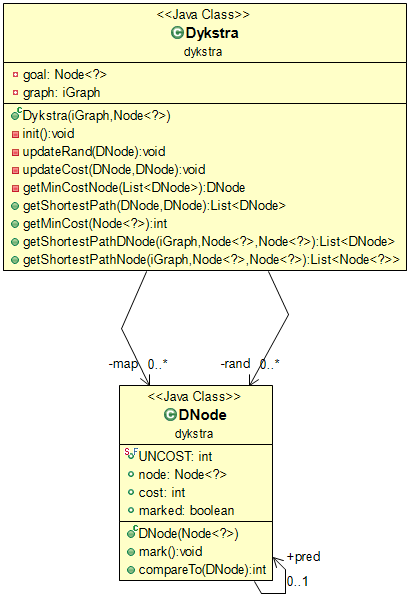
\includegraphics[width=0.5\textwidth]{./IMG/dykstra.png}
    \caption[shortone]{UML Diagramm der Dykstra Implementierung}
    \label{fig:plot}
\end{figure}


\subsection{Zählerintegration}
Aufgrund von Zeitgründen wurde kein schlaues Pattern für die Zählerintegration verwendet. Er wurde deswegen einfach in die innersten Schleifen eingefügt. Es wurden nur die Graphenmethoden \texttt{getNeigbors()} und \texttt{getWeight()} getrackt, da diese im Dykstra verwendet werden.

\section{Messung}
Für die Messung wurde wegen Resourcenknappheit nur bis $10^3$ gemessen, dafür aber die drei ersten Knoten genommen und aus deisen der Mittelwert genommen.
Zum Graphen selber ist zu sagen, dass jeder Knoten zu 50\% der andern Knoten eine verbindung ausweist. 


\begin{figure}[htp]
  	\centering
    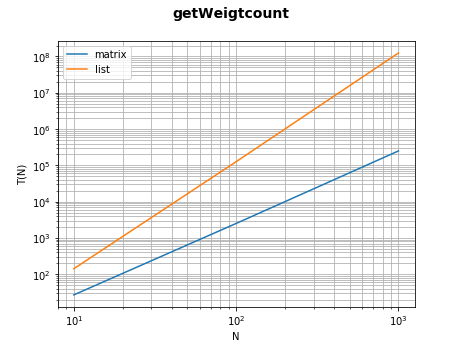
\includegraphics[width=\textwidth]{./IMG/getWeigtcount.png}
    \caption[shortone]{Durchläufe der inneren Schleife von 
    getWeight() während Pathfindung mit Dykstra in Abhängigkeit von 
    der Knotenanzahl N}
    \label{fig:weight}
\end{figure}
\begin{figure}[htp]
  	\centering
    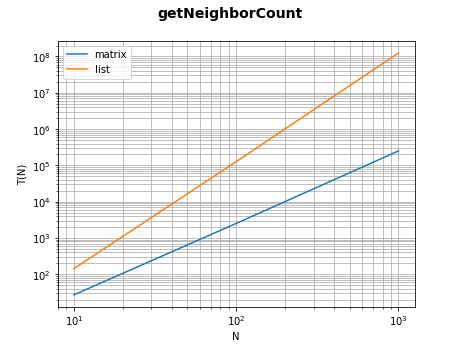
\includegraphics[width=\textwidth]{./IMG/getNeighborCount.png}
    \caption[shortone]{Durchläufe der inneren Schleife von 
    getNeighbors() während Pathfindung mit Dykstra in Abhängigkeit von 
    der Knotenanzahl N}
    \label{fig:neighbor}
\end{figure}
\begin{figure}[htp]
  	\centering
    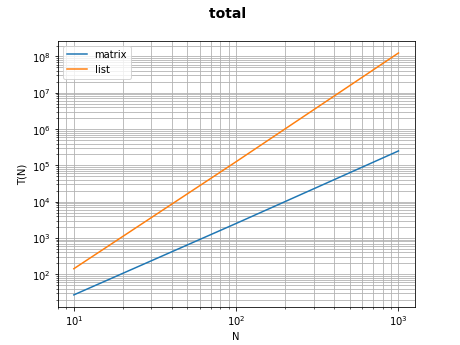
\includegraphics[width=\textwidth]{./IMG/total.png}
    \caption[shortone]{getNeighbors() + getWeight()}
    \label{fig:total}
\end{figure}

Auf den ersten Blick sehen alle Abbildung \ref{fig:weight}, \ref{fig:neighbor}  und \ref{fig:total} gleich aus, dies liegt aber an der logarithmischen Darstellung. Die der Algorithmus mit dem Listengraphen weißt eine Komplexität von $O(n^3)$ und die mit dem MatrixGraphen $O(n^2)$. Dies ist ein wenig widererwartend, da von der Liste eine schnellere Rückgabe der 
Nachbarn erwartet wird.
Eventuell haben wir uns hier vertan. 


\section{Anhang}
Es ist das Javadoc für die Documentation des Codes zu betrachten.
\end{document}
% vim: set spell spelllang=de :EOF
